
\section{Extended taxonomy similarity (ETS) functions and algorithms}

From the TS funciton in the previous section, we saw the utilization of taxonomy trees for the semantic measurement of string similarity, and this funciton are more efective than the traditional syntactic similarity. However, the TS similarity function needs to match the whole string with a single node in the taxonomy tree. But in many cases, such as one record ``California and Michigan'', we cannot match the string with only one term. Therefore, in this section we extend the similarity function to cope with more complicated situations.






\subsection{ETS functions}




\begin{definition}[intersection weight]
Given two token sets $S$ and $T$, and a taxonomy $\mathcal{T}$, we define  an intersection weight $w(e)$ for an element (token) $e \in S$,  if $e \in S_1 \bigcap S_2$, then $w(e)$ = 1; else
 
 \begin{equation}
w(e)=  \max \limits_{e \subseteq S' \subseteq S, T' \subseteq T} ST(S',T',\mathcal{T})
\end{equation} 

\end{definition}


%\noindent \textbf{Remark.}  Given two strings $s$ and $t$, it is clear that $|s \cap t| \leq min (|s|,|t|)$. But based on the taxonomy intersection, it is possible that $|s \cap_T t| > |s| $ or $|s \cap t| > |t| $. For example, s=``California'', t=``U.S.'', $|s \cap_T t|$ = 2. But it is still true that $|s \cap_T t| < |s \cup t|$


We define the taxonomy similarity between two strings as follows:


\begin{definition}[Extended Taxonomy Similarity]   Given two sets of tokens $S$ and $T$,  Let $W_S$= $\sum_{\forall s_i \in S} e(s_i)$ and $W_T$= $\sum_{ \forall t_i \in T} e(t_i)$. Let $Z_S$ and $Z_T$ denote the size of the set of tokens whose weights are zero in $S$ and $T$, respectively.
\begin{equation}
ETS(S,T)=  \frac{min(W_S,W_T)}{min(W_S,W_T)+Z_S+Z_T}
\end{equation} \end{definition}




There are two properties about this extended similarity: (1) \textit{Consistency with Jaccard}: if there are no taxonomy, the  similarity is the same as the Jaccard similarity; (2) \textit{dissimilarity preservation}: given two strings s and t, suppose that the non-overlapping terms (for tokens and taxonomy between s and t is N, then $ETS(s,t) \leq 1- \frac{|N|}{|S|}$. That means, the similarity between two strings cannot be too large if they have enough number of dissimilarity tokens. We can exploit this crucial property for our filtering strategy later.

\begin{algorithm}
{\bf Input}: two strings $s_1$ and $s_2$, a taxonomy $\mathcal{T}$ \\
{\bf Output}: $TJ(s_1,s_2,\mathcal{T})$
\begin{compactenum}[(1)]
\item Let $S_T $ to contain all tokens for taxonomy-based intersection. Initially, $S_T = \emptyset$.
\item Let $L_1$ (resp. $L_2$) denote the applicable taxonomy node list for $s_1$ (resp. $s_2$);
\item Scan $L_1$ and $L_2$ sequentially to find any matching pair $n_1 \in L_1$, $n_2 \in L_2$, s.t. ($n_1$,$n_2$) has the IS-A relation in $\mathcal{T}$;
\item Add all tokens $t \in n_1 \cup n_2$ to the set $S_T$;
\item  return $\frac{S_T \cup (|s_1 \cap s_2|)}{|s_1 \cup s_2|}$;
\end{compactenum}
\caption{String joins with taxonomy}
\label{alg:exactjoin}
\end{algorithm}

The time complexity of the TJ is $O(|s_1|+|s_2|+|n_1|+|n_2|)$, where $n_1$ (resp. $n_2$) denotes all applicable taxonomy nodes for string $s_1$  (resp. $n_2$). Assume that the preprocessing step finds the taxonomy relation for each string. Then the online algorithm only needs to find the matching IS-A relation between two strings to compute the intersection set with taxonomy.

\subsection{String similarity join algorithms}


%\begin{figure}[t]
%\centering
%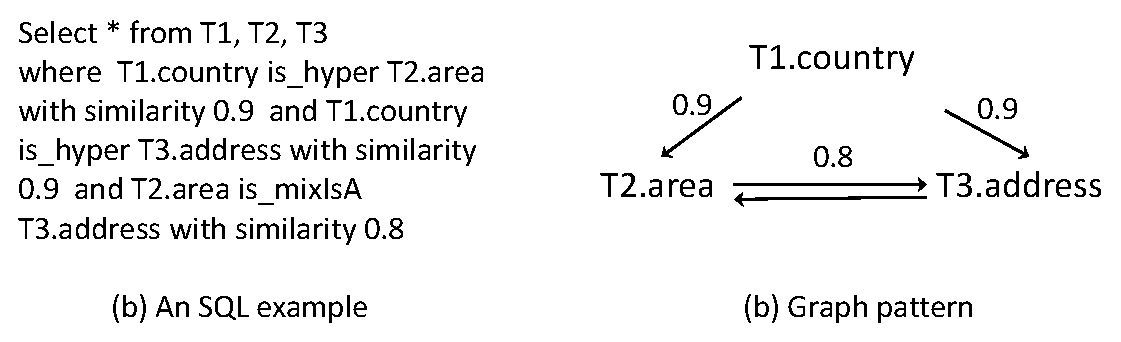
\includegraphics[scale=0.4]{figures/tgsql2}
% \caption{Taxonomy graph example }
%\label{fig:similaritygeaph}
%\end{figure}



\textbf{Baseline algorithm}. We can use the similar algorithm as that in string exact join with taxonomy. And then use these candidate for filtering. But this baseline algorithm has one limitation that there are too many candidates. Then we show how to perform the second filtering to reduce the number of candidate pairs.

\textbf{Signature-based index}. Given a string s with length $|s|$, then the size of signature is $\lceil (1-\theta)|s| \rceil$. But if the signatures involve the taxonomy, then we cannot make this argument.

But if in some real cases, we select the word from taxonomy as signatures. Therefore we need to compute a relax maximum similarity. In this case, we still do not need to retrieve the whole string to compute real similarity.

Given as string $s$, assume that its applied taxonomy node is $n$.

In this paper, we propose a new index which combine a signature filters and a length together with a bit-matrix, which extends bloom filter to two dimensions.

In the literature, the current "modus operandi" is called \textit{prefix filter}, which is based on the intuition that if two canonicalized records are similar, some fragments of them should overlap with each other, as otherwise the two records
won't have enough overlap. This intuition can be formally captured by the prefix-filtering
principle \cite{conf/icde/ChaudhuriGK06} rephrased below.

\begin{lem} (\textsc{Prefix filter principle}) \cite{conf/icde/ChaudhuriGK06} Given an
ordering $O$ of the token universe $U$ and two strings $s$ and $t$, each with tokens sorted in the
order of $O$.   If Jaccard($s, t$) $> \theta$, then the first $\lceil(1-\theta)|s|\rceil$ smallest
tokens of $s$ and the first $\lceil(1-\theta)|t|\rceil$ smallest
tokens of $t$  must share at least one token.
\end{lem}

\subsubsection{N-ary prefix scheme}




Given a string $s$, we can construct the $n$-ary prefix token combination as follows:  Given an
ordering $O$ of the token universe $U$, we select $n$ tokens from the first $\lceil (1-
\theta) \cdot |s| \rceil + n -1$ in $s$. Then let $B^s_n$ denote the set to contain all $n$-combinations. That is  $|B^s_n|$= $\binom{(1-\theta)|s|+n-1}{n}$.

\begin{lem} (\textsc{N-ary signature principle}) Given two strings $s$ and $t$ and their n-ary signatures $T^s$ and $T^t$ respectively, if Jaccard($s, t$) $> \theta$, then $T^s \cap T^t \neq \emptyset$.
\end{lem}

Given a string s=\{A,B,C,D,E\}. If we use the prefix filtering, then the signature is A and B. Assume that $\theta$=0.75, (1-0.75)*5=1.25 and $\lceil 1.25 \rceil$=2. But in our bi-tuple scheme, we select two tokens as the signatures, including \{A,B\},\{A,C\},\{B,C\}.

Similarly, we can develop a 3-tuple signature. we select three tokens as the signatures, including $\binom{4}{3}$=4, i.e. \{A,B,C\}, \{A,C,D\}, \{B,C,D\}, \{A,B,D\}.

Furthermore, we can extend to 4-tuple signature, that is $\binom{5}{4}$=4, i.e. \{A,B,C,D\}, \{A,C,D,E\}, \{A,B,D,E\}, \{A,C,D,E\}, \{B,C,D,E\}.

One question is how to select the number $n$ for n-tuple scheme. What is the optimal value of $n$? Let $t= (1-\theta)|s|$, that is, $O((t+n-1)^{n})$. If n is too large, then there are many signatures, it may not be an optimal solution. Therefore, the key point is how to decide a good $n$?


\subsubsection{N-ary prefix scheme with taxonomy}

 Given a string s=\{A,B,C,D,E\}, assume that we use 3-tuple signature, $\binom{4}{3}$=4, i.e. \{A,B,C\}, \{A,C,D\}, \{B,C,D\}, \{A,B,D\}.

For each tokens, there are two cases, that is, it contains a taxonomy word, say $t \in w$. Then we use $w$ to replace $t$. Note that $t$ may belong to multiple taxonomy words. Therefore, ($w_1, w_2, \cdots, w_3$)

Continue the above example, assume that $DE$ = 1.1. Note that $E \in s $, but $E$ does not belong to the signatures. Then the new three signatures:  \{A,C,1.1\}, \{B,C,1.1\}, \{A,B,1.1\}.

\noindent \textbf{Composite signatures} Given a string $s$, a composite signature of $s$, denoted by C-Sig($s$) includes two types of elements $T$ and $N$, where $T$ is a set of tokens and $N$ is a set of T-nodes.

Given an
ordering $O = (U_1 , U_2 )$ of the token universe $U_1$ and $U_2$, where $U_1$ denotes the set of non-taxonomy tokens and $U_2$ is the set of taxonomy tokens. Let $P_s$ denote the smallest $\lceil(1-\theta)|s|\rceil$ tokens.

%\begin{lem} (\textsc{Prefix filter principle with taxonomy})  Given two strings $s$ and $t$ with n-ary prefix signatures, if TJ($s, t$) $\geq \theta$, then one of the following cases holds:
%
% \begin{itemize}
%   \item $P_s \cap P_t \neq \emptyset$, or
%   \item  $T_s \cap A_t \neq \emptyset$ or $T_t \cap A_s \neq \emptyset$
% \end{itemize}
%
%\end{lem}
%


%\begin{lem} (\textsc{Prefix filter principle with taxonomy})  Given two strings $s$ and $t$ with n-ary prefix signatures, if TJ($s, t$) $\geq \theta$, then one of the following cases holds:
%
% \begin{itemize}
%   \item $P_s \cap P_t \neq \emptyset$, or both of the conditions satisfy:
%   \item  $\exists sig^s \in P_s, sig = sig^s_{token} \cup sig^s_{tax} s.t. \exists sig^t \supseteq sig^s$ and $sig^s_{tax} \subseteq Tax(t)$ and
%    \item  $\exists sig^t \in P_t, sig = sig^t_{token} \cup sig^t_{tax} s.t. \exists sig^s \supseteq sig^t$ and $sig^t_{tax} \subseteq Tax(s)$
% \end{itemize}
%
%\end{lem}

A signature set $P$ for a string $s$ is a binary tuple ($T,N$), where $T$ is a set of tokens and $N$ is a set of taxonomy nodes.

\begin{definition} [Signatures match strings]
Given a signature set $P = (T,N)$ and a string $s$, we say $P$ matches $s$, denoted by $P \vdash s$ if $N \subseteq N^s$, where $N^s$ is a set of applicable taxonomy nodes of $s$ and  there exits a signature set $P' = (T',N')$ of $s$, s.t. $T \subseteq T'$.
\end{definition}


\begin{lem} (\textsc{Composite signatures principle})  Given two strings $s$ and $t$ with signatures $P^s$ and $P^t$ respectively, if TJ($s, t$) $> \theta$, then $P^s \vdash t$ and $P^t \vdash s$.

\end{lem}

For example, consider two strings s=\{A,B,C,D,E\} and t=\{F,G\}. Assume that $t_1$ = (ACD,G) is an IS-A relation and the $|s \cap_T t| $=4, $JT(s,t)$ = $\frac{4}{7}$= 0.57.
If the threshold $\theta =$ 0.5, then  $\lceil (1-\theta) \times 5 \rceil$= 3 for $s$ and $\lceil (1-\theta) \times 2 \rceil$= 1. Assume that the order of non-taxonomy tokens $O_1$= \{$B, E, F$\} and the order of taxonomy tokens is $O_2$ = \{$A, C, D, G$\}. So the signature of $s$ is \{B,E,A\}, and an IS-A relation $T_s$ = (ACD,G). The signature of $t$ is \{F\} and $A_t$ = (ACD,G). $ T_s \cap A_t \neq \emptyset$.

\subsubsection{Similarity join algorithm}

We discuss the similarity join algorithm based on the above n-ary composite signature filters.


\begin{algorithm}
{\bf Input}:  two collections of strings $S$ and $T$ and the threshold $\theta$ \\
{\bf Output}: result pairs ($s,t$)$\in S \times T$, s.t. JT($s,t$)$> \theta$
\begin{compactenum}[(1)]
\item Find candidate pairs $C_1$ = \{$(s,t) |$  $P^s \vdash t$\};
\item Find candidate pairs $C_2$ = \{$(s,t) |$  $P^t \vdash s$\};
\item  $C= C_1 \cap C_2$;
\item FOR EACH ($s,t$)$\in C$
\item RETURN all pairs s.t. $JT(s,t) > \theta$
\end{compactenum}
\caption{String joins with taxonomy}
\label{alg:exactjoin}
\end{algorithm}

For each table, we can generate four inverted lists for strings: (1) a list $L_I$ for tokens where the signatures of strings contain only tokens; (2) a list $L_{II}$ for taxonomy nodes where the signatures of strings contain only nodes; (3) a list $L_{III}$ for tokens where the signatures of strings contain both tokens and nodes; (4)  a list $L_{IV}$ for nodes where the signatures of strings contain both tokens and nodes.


\begin{algorithm}
{\bf Input}: two collection of strings $S$ and $T$ and their corresponding inverted lists $L_I^S$,  $L_{II}^S$, $L_{III}^S$, $L_{IV}^S$, $L_N^T$ \\
{\bf Output}: string candidate pairs \{$(s,t) |$  $P^s \vdash t$, $s \in S$ and $t \in T$\}
\begin{compactenum}[(1)]
\item  $C_1$=$\displaystyle\bigcup_{g \in L_I^S \cap L_I^t} (L_I^s(g) \times L_I^t(g)) $;
\item  $C_2$=$\displaystyle\bigcup_{n \in L_{II}^S \cap L_N^t} (L_{II}^s(n) \times L_N^t(n)) $;
\item  $C_3$=$\displaystyle\bigcup_{g \in L_{III}^S \cap L_{III}^t} (L_{III}^s(g) \times L_{III}^t(g)) $;
\item  $C_4$=$\displaystyle\bigcup_{n \in L_{IV}^S \cap L_N^t} (L_{IV}^s(n) \times L_N^t(n)) $;
\item   Return $C_1 \cup C_2 \cup (C_3 \cap C_4)$;

\end{compactenum}
\caption{String candidate pairs}
\label{alg:exactjoin}
\end{algorithm}

\begin{table*}[t]
\centering
\begin{tabular}{|@{\hspace{1mm}}c@{\hspace{1mm}}|@{\hspace{1mm}}c@{\hspace{1mm}}|}
%{|p{1cm}|p{1cm}|p{1cm}|p{1cm}|p{1cm}|p{1cm}|p{1cm}|}
%|c|m{6cm}|
\hline
 \textbf{Symbols} & \textbf{Definitions}  \\
  \hline \hline

  $L_I(g)$ &    $\forall s \in L_I(g)$,  s.t. $\exists  R  \in C$-$Sig(s)$, $R$ contains only tokens and $g \in R$ \\

   $L_{II}(n)$ & $\forall$ $s \in L_{II}(n)$, s.t. $\exists  R  \in C$-$Sig(s)$, $R$ contains only T-nodes and $n \in R$    \\

   $L_{III}(g)$ & $\forall$ $s \in L_{III}(g)$, s.t.  $\exists R  \in C$-$Sig(s)$, $R$ contains both tokens and T-nodes, $g \in R$    \\

  $L_{IV}(n)$ &  $\forall s \in L_{IV}(n)$, s.t. $\exists R  \in C$-$Sig(s)$, $R$ contains tokens and T-nodes and $n \in R$    \\

$L_{N}(n)$ &  $\forall s \in L_{N}(n)$, s.t. $n$ is an applicable T-node of $s$   \\

  \hline
\end{tabular}
\caption{Summary of definitions of various inverted lists}
\label{tab:symbols}
\end{table*}


\begin{table*}[t]
\centering
\begin{tabular}{|@{\hspace{1mm}}c@{\hspace{1mm}}|@{\hspace{1mm}}c@{\hspace{1mm}}|@{\hspace{1mm}}c@{\hspace{1mm}}|@{\hspace{1mm}}c@{\hspace{1mm}}|}
%{|p{1cm}|p{1cm}|p{1cm}|p{1cm}|p{1cm}|p{1cm}|p{1cm}|}
%|c|m{6cm}|
\hline
 \textbf{ID} & \textbf{Strings} &  \textbf{Signatures} &    \textbf{C-Sig} \\
  \hline \hline

  $q_1$ & Suwon and Seoul in South Korea  &  (Suwon, and), (Suwon Seoul), (and, Seoul)  & (3.1.1.2, and), (3.1.1.2, 3.1.1.1), (and, 3.1.1.1) \\

   $q_2$ & Seoul, South Korea in Asia  & (Seoul, South), (Seoul, Korea), (South, Korea) &   (3.1.1.1, 3.1), (3.1.1.1, 3.1), (3.1, 3.1) \\

   $q_3$ &  two states: California and Michigan, U.S. &  (two, states), (two, California), (states, California) & (two, states), (two, 2.1.1), (states, 2.1.1)  \\
   $q_4$ & two cities: Detroit and Los angles & (two, cities), (two, Detroit), (cities, Detroit) &  (two, cities), (two, 2.1.2.1), (cities, 2.1.2.1) \\


  \hline
\end{tabular}
\caption{An example to illustrate the string similarity join algorithm}
\label{tab:example}
\end{table*}


\begin{example} We use Table as an example to illustrate the algorithm.

\end{example}

\subsubsection{Comparison with other schemes}


\begin{table}[t]
\centering
\begin{tabular}{|@{\hspace{1mm}}c@{\hspace{1mm}}|@{\hspace{1mm}}c@{\hspace{1mm}}|@{\hspace{1mm}}c@{\hspace{1mm}}|}
%{|p{1cm}|p{1cm}|p{1cm}|p{1cm}|p{1cm}|p{1cm}|p{1cm}|}
%|c|m{6cm}|
\hline
 \textbf{Methods@{}} & \textbf{Signature size} &  \textbf{Filtering power} \\
  \hline \hline

  Prefix & (1 -$\theta$)$|s|$ & Optimal \\


   PartEnum & CPU:  O($1.2002^{|V|} \cdot |V|^{O(1)}$ ) & Optimal \\

   LSH & CPU:  O($|V|$log$|V|$+$|E|$)  & $(2\bar{d}+3)/5$  \\

   Composite Prefix & I/O: O(sort($|E|$+$|V|$))   & No bound \\


  \hline
\end{tabular}
\caption{Time and  I/O cost and performance}
\label{tab:complexity}
\end{table}

 We compare our composite prefix filter with state-of-the-art filters. The objective of the filters is to prune dissimilar strings as many as possible. They require to select a set of q-grams from each of two strings as signatures, denoted as Sig(r) and Sig(s), and compare the two q-gram sets to check whether they share common signatures. Pruning power and filtering cost are two important issues in designing filters.

We first consider the pruning power. One one hand, the smaller the production size of the two signature sets $|Sig(r)| \times$
$|Sig(s)|$, the smaller probability they share common q-grams, and thus the higher pruning power. On the other hand, the number of matching q-grams cannot exceed the smaller signature size of the two strings, min($|Sig(r)|, |Sig(s)|$). Thus
we can use the production size of two signature sets and
the smaller signature set size to evaluate the pruning power. We then evaluate the filtering cost. As the q-gram sets
are sorted, we can use a merge-join algorithm to find the
matching q-grams if there is no index, the filtering cost depends on the sum of signature set sizes of the two strings,
$|Sig(r)|$ + $|Sig(s)|$. Table 3 compares the pruning power and filtering cost of state-of-the-art q-gram-based filters used in AllPair, ED-Join, Qchunk-IndexChunk and Qchunk-IndexGram.

\smallskip

\noindent \textbf{Length filters}


\subsubsection{Composite signature: Performance}

In this section, we cover various aspects of Composite-signature scheme's performance.
We begin by proving that it has good asymptotic performance: For a particular setting of n1 and n2, we can prove
that it provides good filtering effectiveness (i.e., generates only a few false positive candidate pairs) with few signatures per input set.

\begin{theorem} If the Jaccard similarity of two strings are greater than $\theta$, then $Sig(u) \bigcap Sig(v) = \varnothing$ with probability 1-o(1). For this setting of parameters, the number of signature per string is O().
\end{theorem}


Given a $n$-tuple composite filter, we estimate its filtering effectiveness.

We assume that there are $N$ tokens in all tables and the length of each string is $s$.

The possibility of false positive for a string pair $s, t$ is that $P(E_A | E_B)$, $E_B$ means that  $sim(s,t) < \theta$; $E_A$ means that $s$ and $t$ pair cannot be pruned away with the filter.

First consider the 1 prefix signature. We computer $P(E_A, E_B)$, that is, the prefix signature cannot prune away the pair of $Jaccard(s,t) < \theta$

Let $\lambda$ = $(1-\theta)s$ signatures for $t$.

Since $|s| = |t|$ and   $Jaccard(s,t) < \theta$ $\Longleftarrow$ $ |s \cap t| < |s| \cdot \theta$.

%\subsection{Count-Min estimation}
%
%In order to quickly decide if the number of pairs after composite filters, we develop a count-min estimation to quickly determine which $n$ is good for filtering. See the following two examples for joins.
%
%See the example in Figure \ref{fig:signature_example1}. In this example, $\theta$ = 0.8. If we use the 1-element signature, then we cannot prune away any string pair. In signature 2, we use 2-element signature, then there is no candidate. Therefore, the filtering power is better.
%
%Further, when we consider the taxonomy ABCD ISA AGK, shown in Figure \ref{fig:signature_example1}. Then there is one answer pair (s1,t1). The new signature include the taxonomy ID 1.1 and 1  as shown.
%
%\begin{figure}[h]
%\centering
%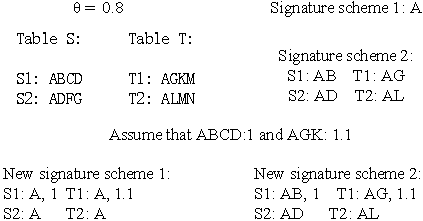
\includegraphics[scale=0.8]{figures/signature_example1}
% \caption{Illustration to the difference of signature schemes}
%\label{fig:signature_example1}
%\end{figure}
%
%A Count-Min (CM) sketch with parameters ( $\varepsilon, \delta$) is represented by a two-dimensional
%array counts with width $w$ and depth $d$. Given parameters ($\varepsilon, \delta$), set
%$w$ = $\lceil \frac{e}{\varepsilon} \rceil$ and $d$ = $\lceil ln \frac{1}{\delta} \rceil $. Each entry of the array is initially zero.
%
%
%When a data item ($w,i$) arrives, meaning that the signature $w$ has the length $i$, then $i$ is added to one cell in each row; the counter is determined by $h_j$. Formally, set $\forall 1 \leq j \leq d$, then count[j,$h_j(i)$]
%
%
%The space used by Count-Min sketches is the array of $wd$ counts, which takes $wd$ words, and $d$ hash
%functions, each of which can be stored using 2 words when using the pairwise functions described in [27].
%
%Estimation procedure. Our estimation for $S \bigodot T $ = $min_j S_j \bigodot T_j $
%
%
%\begin{theorem}
%With a probability 1- $\delta$, The upper bound and lower bound of Composite signature estimation is
% $S \bigodot T $ and  $S \bigodot T $ + $\varepsilon |S| |T|$, respectively.
%\end{theorem}
%
%\begin{theorem}
%Our composite signature estimation estimates the lower and upper bounds of algorithms by keeping space $O(\frac{1}{\varepsilon} \log \frac{1}{\delta})$ and
%\end{theorem}
%
%\subsubsection{Estimation with length filters}
%
%When we use the CountMin sketch to estimate the effectiveness of length filter. It is to



\subsection{Extensions for flexible query thresholds} \label{subsec:flexible}

In the previous sections, our model assumes that the search threshold is fixed, and only the query can be changed online. However, in practice users might change the threshold at query-time. Therefore, we now move to a more general case, where both the search string and the threshold are flexible at query-time. The new challenge here is that we do not know the threshold in advance and thus we cannot determine the number of signatures of each record. A na\"{i}ve method is to compute the signatures of records in the table online according to the given threshold, which  is clearly prohibitively expensive. Next we build a new index called \textit{FSI-trees} (Flexible Signature Indexing) by extending SI-trees to solve this problem.

Suppose that all meaningful thresholds distribute in the range between 0.99 to 0.50. Then we select some \textit{representative thresholds}, e.g. 0.95, 0.90, etc.   For each representative threshold, we generate signatures for each record. See an example in Figure \ref{fig:FSI}(a). Note that the signatures of a string for lower thresholds are guaranteed to become signatures of that for higher thresholds. To build an FSI-tree,  the length and fence entries of SI-trees remain the same. But each fence entry points to a set of I-lists which come from \textit{all} representative thresholds. Further, each element in the I-list of a signature token $s$ is a binary tuple ($q$, $\theta$), where $q$ is a record ID and $\theta$ is the minimal threshold for which this signature $s$ appears in $q$. For example, in Figure \ref{fig:FSI}(b), the token ``\textsf{Computing}''  is a signature of $q_1$ for all thresholds $\geq 0.5$.

We extend the QP-search algorithm for flexible thresholds. The algorithm almost remains the same, but  the only  change (See Algorithm \ref{algo:QP-flexible}) is that we select the string candidates in I-lists by checking their thresholds (Line 3).

An astute reader may notice that our method possibly introduces more candidates because of the gap between representative thresholds and online thresholds. For example, given a query threshold 0.83, suppose that the closest representative threshold is 0.80. Then  the number of signatures for threshold 0.80  may be greater than that for 0.83. But we argue that the problem  has actually a little impact on the final performance of query processing. To understand this, assume that gap between two representative thresholds is no more than 0.05 (that means, only 11 representative thresholds are ``materialized'' with signatures between 0.99 and 0.50). It can be proved that given a string $s$, the difference between the numbers of signatures for thresholds $\theta_1$ and $\theta_2$ is $\lceil  |\theta_1 - \theta_2|   \cdot |s| \rceil$. Considering a string $|s|$=10, we have 0.05 * 10 =0.5, That is, for most records in the table, the extra number of signatures due to the thresholds gap  is bounded by 0.5. Therefore, as our experimental results show in Section \ref{subsec:searchalgorithms}, the performance of our algorithms for flexible thresholds is comparable to that for static thresholds.



